\documentclass[12pt,twoside,a4paper]{article}


\usepackage[utf8]{inputenc}
\usepackage[T1]{fontenc}
\usepackage{lmodern}

% Quelques packages utiles
\usepackage{listings} % Pour afficher des listings de programmes
\usepackage{graphicx} % Pour afficher des figures
\usepackage{amsthm}   % Pour créer des théorèmes et des définitions
\usepackage{amsmath}
\usepackage{microtype} % Optical margins FTW
\usepackage{url}
\usepackage{booktabs} % Allows the use of \toprule, \midrule and \bottomrule in tables for horizontal lines
\usepackage[per-mode=symbol]{siunitx}
\usepackage{floatrow}
\usepackage{caption}
\usepackage{subcaption}
\usepackage{fullpage}
\usepackage{rotating}
\usepackage{lipsum}
\usepackage[space]{grffile}

%table of content link to the section
\usepackage{hyperref}
\hypersetup{
    colorlinks,
    citecolor=black,
    filecolor=black,
    linkcolor=black,
    urlcolor=black
}

\newcommand{\ts}{\textsuperscript}

\title{System Engineering: Pedometer on pebble watch}
\author{Antoine Albertelli \and Eloi Benvenuti \and Florian Kaufmann}
\date{October 2016}

% Début du document

\begin{document}
\maketitle

\section{Introduction}
In the context of our System Engineering class we had to design and code a pedometer for a pebble smart	watch. This document explains our design process and presents the final results
\section{Requirements}
The need tied to the user of pedometer are the following:
\begin{itemize}
	\item Have a mean to count his footsteps over the day.
	\item Have a mean to easily read his current footsteps for the day.
	\item Have a mean to access an history of his footsteps over the past days.
	\item Must not experience discomfort due to the use of the device.
\end{itemize}

From those needs we derived the following functions:
\begin{enumerate}
	\item Acquire the relevant data for footsteps computing.
	\item Process those data to compute the number of footsteps.
	\item Update the number of footsteps frequently (every 1-2 seconds).
	\item Display the number of footsteps for the current day.
	\item Offer a mean to reset the current number of footsteps.
	\item Is able to count footsteps in the background.
	\item Offer a mean to look at the history of footsteps for the past week.
	\item Do not reduce the battery life of the pebble watch noticeably.
	\item Do not result in an overheating of the watch.
\end{enumerate}

\section{Algorithms}
We tried several approaches in order to find a precise enough algorithm.
We implemented prototype in Matlab or Python and ran them on the sample data.
We then compared the number of counted step against the actual number of steps in order to rank them.

\subsection{Frequency domain}
We briefly explored the idea of processing the data in the frequency domain.
The approach we used was to cut the frequencies above and below a certain signal and look for peaks in the frequency spectrum.
However we rejected this idea because of the complexity and computational costs compared to the time domain algorithm (see below).

\subsection{Time domain}
We implemented 3 time domain algorithms and compared them against each other.

Here is a quick description of their different strategy:
\paragraph{Algorithm 1}
The 1\ts{st} implementation looks at the data by blocks of 1 second.
If the peak-to-peak difference was bigger than a set threshold the step counter is incremented.
This algorithm had good performance on the test data but was discarded because it was too sensitive to the walking pace:
If multiple steps fit in the data block only one step would be counted.

\paragraph{Algorithm 2}
The 2\ts{nd} implementation counts the steps using the data of the three axis of the accelerometer.
Its strategy, applied separately to each axis, was to find the average value of the data in the block
It would then count one step every time the raw data crossed the average with a negative slope.
In order to reduce miscounts due to the noise, an hysteresis was applied.

This algorithm performed very badly, overshooting the number of steps by a factor 2 at least.
The averaging between the 3 axis wasn't helping, since the 2 worst-performing axis were only worsening the count of the "best" axis.

\paragraph{Algorithm 3}

\begin{figure}[h]
    \centering
    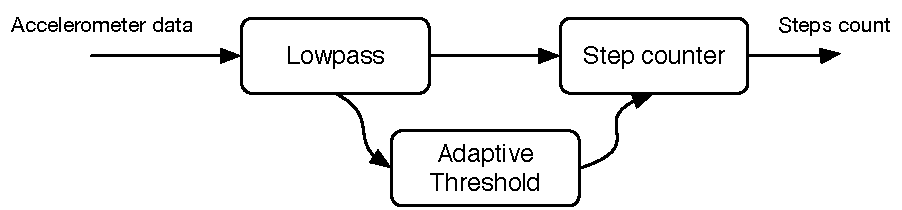
\includegraphics{algorithm}
    \caption{Final version of our algorithm}
    \label{fig:algorithm}
\end{figure}

The final algorithm (fig. \ref{fig:algorithm}) count the steps using only 1 axis.
It first applies a lowpass filter on the data to smooth out the noise.
It then compares the data to a threshold calculated using an average over the last N points.
When the data crosses the threshold (with an hysteresis), one step is counted.
Compared to the previous algorithm, this result in a threshold reacting more smoothly which improves the precision.

Its performance is very good: on test data, it is within 10\% of the correct value.
Moreover, it is easy to implement correctly, doesn't consume a lot of processing power nor RAM and only has a few parameters to tune (filter frequency, threshold history size and hysteresis).
It is also pretty insensitive to variations in physical parameters across users.

\begin{figure}[h]
    \centering
    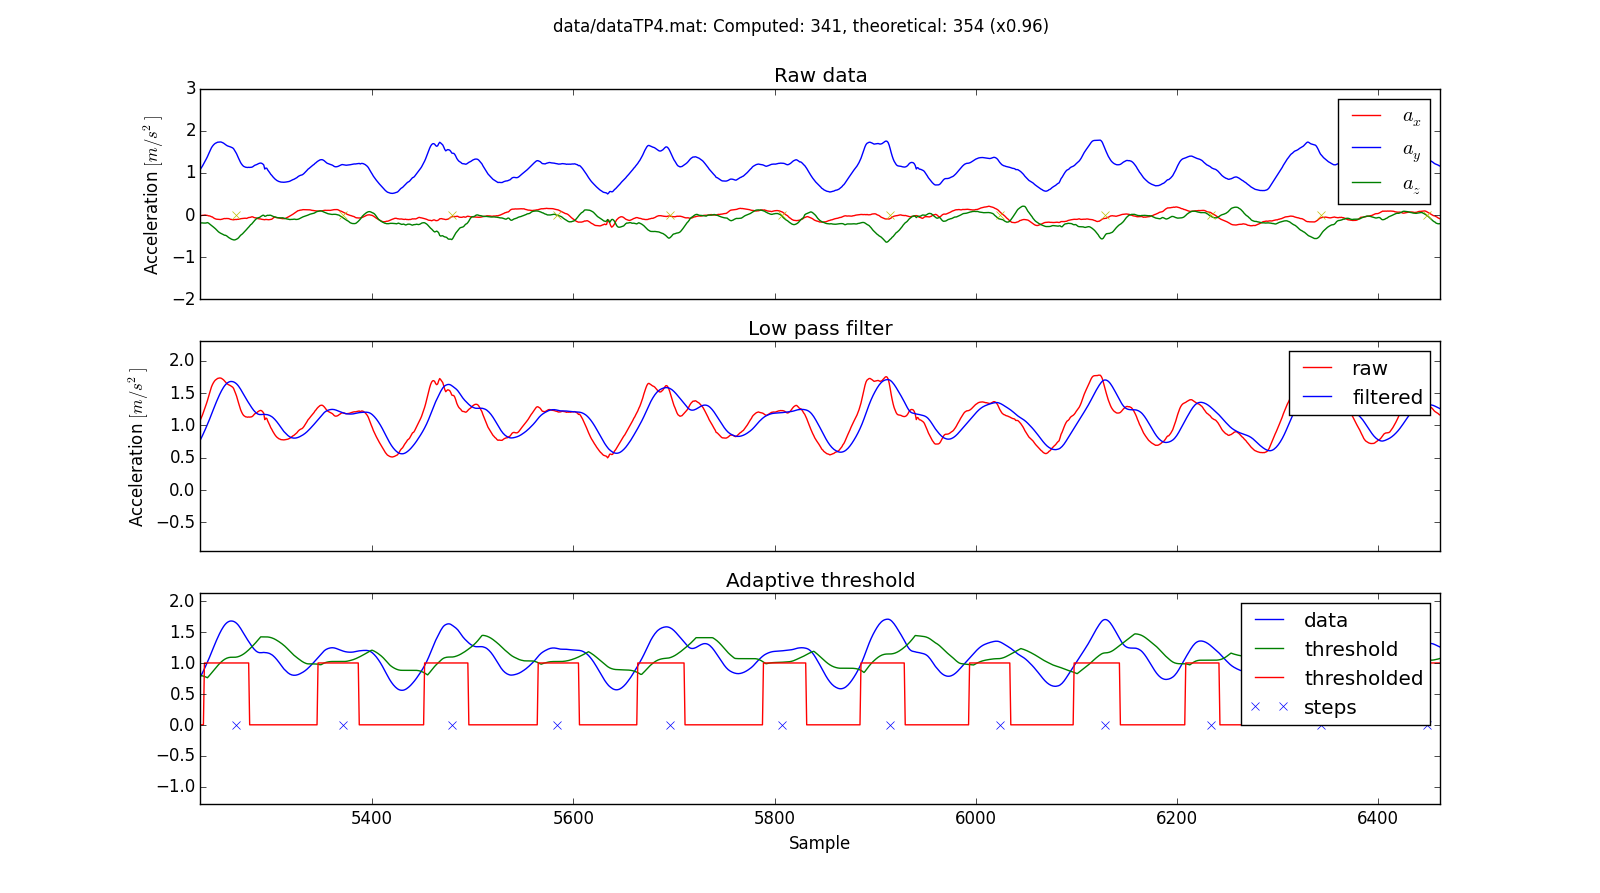
\includegraphics[width=0.8\textwidth]{algorithm_steps}
    \caption{Processing steps of our final algorithm.
        First, the raw data (top) pass through a low pass filter to reduce noise (middle).
        Finally the threshold is compared to the filtered data and a step is counted on every crossing (bottom).
    }
    \label{fig:steps}
\end{figure}

\section{Implementation notes}
The processing code was first written in Python, then in C.
The code was written to be very portable by separating platform-dependent code from processing functions.
This allows the code to be tested on a development machine, which increases development velocity.

We also wrote some unit tests for the processing code (under the ``tests'' folder).
This prevents bug and reduces time spent debugging on the Pebble.

In order for the user to be still able to use his watch while having the pedometer on we implemented a background worker who is in charge of counting the steps.
This separation allows the user to go on the main window of the application only to check his current number of steps and then leave the app to use other functions.
This is, a critical function of the pedometer because no one is going to use an application that requires one to stop using all the other application of the watch.

To communicate between the worker and the application a message queue is provided by the Pebble API.
We implemented three messages for our use cases:
\begin{enumerate}
    \item The worker sends the step count and the current state (turned on or off) to the application.
        This is used to update the screen.
    \item The application sends one message to toggle the state between on and off to the worker.
    \item The last message type is sent from the application to the worker to reset the step counter to zero.
\end{enumerate}

\section{Interface design}
Figure \ref{fig:interface} shows a screenshot of the interface when the pedometer is running. We wanted to display the 
minimum amount of infos while still providing the user with the necessary ones in order to instantly know how much 
steps he had already walked and the functions of the different buttons. In order to communicate them we used commonly 
known symbols such as small ``play'' and ``pause'' icons for the top button and circling arrows for the bottom one, 
used to reset the count.
\begin{figure}[h]
    \centering
    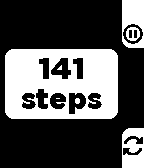
\includegraphics{screenshot}
    \caption{Screenshot of our interface showcasing the reset and play/pause button}
    \label{fig:interface}
\end{figure}


\end{document}
